\documentclass[10pt,a4paper]{article}
\usepackage[utf8]{inputenc}
\usepackage[T1]{fontenc}
\usepackage{lmodern}
\usepackage[margin=1.5cm, top=1.4cm, bottom=1.4cm]{geometry}
\usepackage{hyperref}
\usepackage{enumitem}
\usepackage{titlesec}
\usepackage{xcolor}
\usepackage{graphicx}

\definecolor{accent}{HTML}{1F4E78}
\hypersetup{colorlinks=true, urlcolor=accent, linkcolor=accent}
\pagenumbering{arabic}
\setlength{\parindent}{0pt}

\titleformat{\section}{\large\bfseries\color{accent}}{}{0em}{}[\vspace{-0.6em}\rule{\textwidth}{0.8pt}]
\titlespacing{\section}{0pt}{7pt}{4pt}

\newcommand{\role}[4]{%
  \textbf{#1} \hfill \textbf{#2}\\[1pt]%
  \textit{#3} \hfill \textit{#4}\\[2pt]%
}
\setlist[itemize]{leftmargin=1.2em, itemsep=1.5pt, topsep=2pt, parsep=0pt}

\begin{document}

% ================= HEADER =================
\begin{minipage}[c]{0.80\textwidth}
  {\Huge\bfseries Prabhavit Gupta}\\[3pt]
  {\color{accent}\large AI Architect / Solutions Engineer: Agentic Systems, RAG \& API Orchestration}\\[6pt]
  {\footnotesize +39 351 610 7807 ~$\vert$~
  \href{mailto:prabhavitg@gmail.com}{prabhavitg@gmail.com} ~$\vert$~
  \href{https://www.linkedin.com/in/prabhavit/}{linkedin.com/in/prabhavit} ~$\vert$~
  \href{https://github.com/prab-gupta}{github.com/prab-gupta} ~$\vert$~
  Venice, Italy}
\end{minipage}\hfill
\begin{minipage}[c]{0.18\textwidth}
  \raggedleft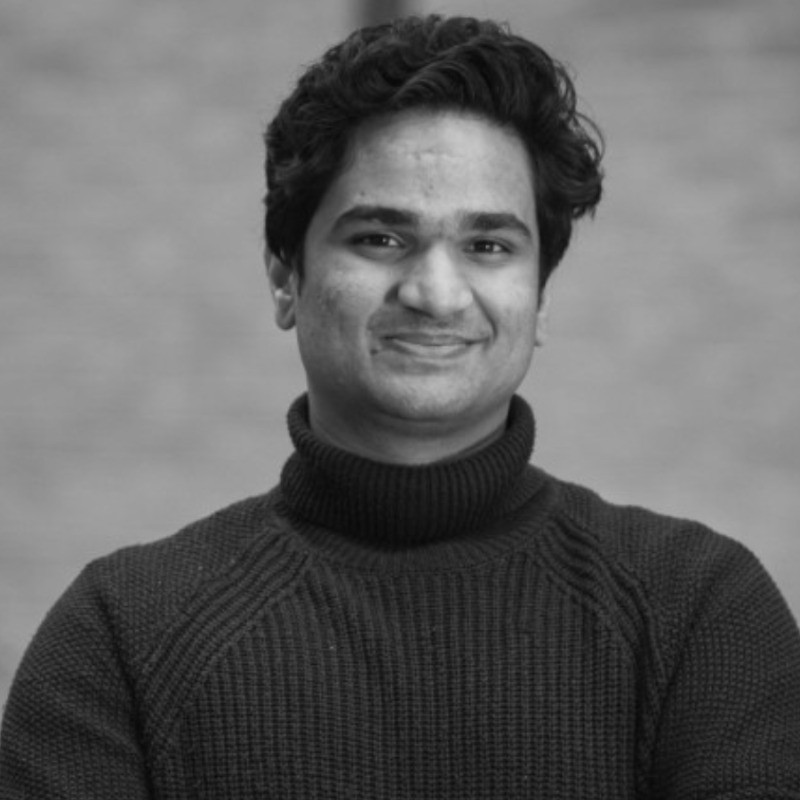
\includegraphics[width=2.0cm]{photo.jpg}
\end{minipage}
\vspace{-2pt}

% ================= SUMMARY =================
\section{Summary}
AI solutions engineer and technical architect with 3 years of hands-on commercial experience designing, building, and deploying production-grade LLM applications, agentic workflows, and knowledge retrieval pipelines. As Lead Developer at FlowSpace, architected multi-step customer support agents with tool use and live API function calling, end-to-end RAG pipelines with vector databases for automated document parsing, Stripe payment processing integrations, and observability safeguards. Deep expertise directing LLM tool-calling architectures, structured JSON outputs, n8n automations, Claude Code workflows, and robust RESTful integrations with TypeScript and working-level Python. Based in Venice, Italy with an EU Long Term Residence Permit (unrestricted EU right to work without sponsorship). Immediately available.

% ================= TECHNICAL EXPERTISE =================
\section{Technical Expertise}
\begin{itemize}
  \item \textbf{Generative AI \& Agents:} Multi-agent orchestration, Tool Calling, Function Calling, Prompt Engineering, Structured JSON Outputs, Agentic workflows, Model Context Protocol (MCP).
  \item \textbf{RAG \& Retrieval:} Semantic search, Vector databases (pgvector, Supabase), Embeddings, Chunking, Hybrid retrieval, Reranking strategies.
  \item \textbf{Fintech \& API Integrations:} Stripe payment gateways, Webhook listeners, Idempotent transaction processing, REST API architecture, OfficeRnD, Nexudus.
  \item \textbf{LLMOps \& Guardrails:} LLM tracing, Observability, Token and cost optimization, Schema validation, Automated error handling, Human-in-the-loop review.
  \item \textbf{Software Engineering:} TypeScript, Node.js, Working-level Python, PostgreSQL, SQL, Docker, n8n, Playwright, Git, Postman.
  \item \textbf{Languages \& Authorization:} Hindi (Native), English (C1 Professional), Italian (Beginner). EU Long Term Residence Permit (No EU sponsorship required).
\end{itemize}

% ================= EXPERIENCE =================
\section{Experience}

\role{\href{https://flowspace.co}{FlowSpace.co}}{Mar 2024 - Aug 2026}{Lead Developer (Full-time, Freelance)}{London, UK (remote)}
\begin{itemize}
  \item Architected and shipped production customer support AI agents using LLM tool use and function calling against live platform APIs, evaluating confidence scores and escalating complex queries to staff.
  \item Designed an automated AI listing and knowledge ingestion pipeline with human-in-the-loop review: parsed structured property records from heterogeneous documents (PDFs, spreadsheets, unstructured pages) into PostgreSQL/Supabase, drafting 900+ verified listings.
  \item Architected financial and booking integrations: implemented secure Stripe payment flows, webhook transaction reconciliation, and bidirectional booking synchronization with OfficeRnD and Nexudus APIs.
  \item Directed architecture migration off a legacy stack to a modern Next.js, TypeScript, and Laravel backend, establishing API specifications and schema contracts across teams.
  \item Implemented token and cost monitoring, schema guardrails, and automated regression testing using Playwright to ensure high reliability across production endpoints.
  \item Scaled platform user base from 2,000 to 4,500+ active users through iterative architectural improvements and resilient backend automations.
\end{itemize}

\role{Urlink}{Apr 2025 - Jul 2025}{Project Manager \& AI Assisted Developer (Freelance)}{Barcelona, Spain (remote)}
\begin{itemize}
  \item Led architecture and rapid technical delivery of AI-assisted web applications, coordinating API contracts, database schemas, and external service integrations.
  \item Implemented automated testing pipelines and CI/CD verification workflows, reducing deployment regressions and release cycle times.
  \item Evaluated external AI APIs and models for cost, latency, and output consistency, integrating optimal models for client-specific use cases.
\end{itemize}

\role{Independent Technical Consultant}{Aug 2023 - Feb 2024}{AI Solutions \& Automation Engineer}{Venice, Italy}
\begin{itemize}
  \item Built customized AI automation workflows, web scrapers, and data enrichment pipelines for European SME clients using n8n, Playwright, and OpenAI APIs.
  \item Implemented idempotent CRM webhook handlers and automated invoice reconciliation workflows, eliminating manual data entry.
  \item Delivered custom RAG-powered chatbot prototypes integrated with company knowledge bases for automated inquiry triage.
\end{itemize}

% ================= EDUCATION =================
\section{Education}
\role{Ca' Foscari University of Venice}{2020 - 2024}{BA in Philosophy, International Studies and Economics}{Venice, Italy}
\begin{itemize}
  \item Rigorous focus on formal logic, analytical problem solving, systems analysis, and macroeconomic decision models.
\end{itemize}

\end{document}
